% !TEX root = ../Mappe.tex
\documentclass[../Mappe.tex]{subfiles}

\graphicspath{{./Bilden/}}

\begin{document}
\section{Künstliche Intelligenz, Chance oder Risiko?}

\begin{figure}[b]
    
    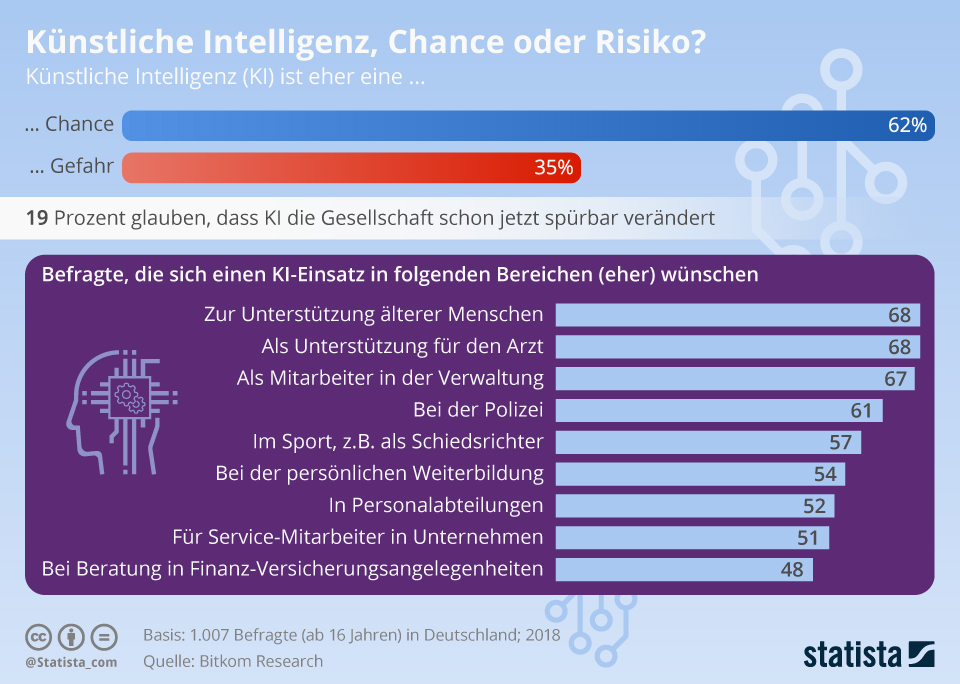
\includegraphics[width=\textwidth]{16394}
    \caption{\cite{kichance}}
    \centering
\end{figure}

Obwohl der nächste große Erfindung Menschheits könnte unsere große Schritt in Technologie seit,
er beinhaltet auch viele Gefahren.

Die unterschiedliche Meinungen werden in eine Grafik, unter der Überschrift "Künstliche Intelligenz, Chance oder Risiko?", representiert.
Dieses Infografik von Statista bearbeitet die Umfragenergebnissen von Bitkom Research.
In die Umfrage nahmen 1007 deutsche Jugendlichen und Erwachsenen teil, wobei sie ihre Standpunkten mittgeteilt haben.
Das Diagramm zeigt uns die grafisch represetierte Antworten auf zwei Fragen.

Zuerst sehen wir wie viele Menschen halten Künstliche Intelligenz eine Gefahr oder eine Möglichkeit.
Die Mehrheit verfügt über ein positiver Zukunftsbild: sie sehen Chance in die neue Technologie.
Etwas über ein drittel der Befragten haben aber ein abere Meinung: sie halten es gefährlich.

Der zweite Säulendiagramm zeigt uns, in welche Bereichen möchten wie viele Menschen die Einführung die KI.
In gleichstand stähen der Hilfe älteren Menschen und KI als Zeug für einen Arst.
Mit genau 20 Prozent weniger Stimmen, in der lätzte Position stäht Finanz- und Versicherungsberatung.
Es ist bemerkenswert, dass das Prozentenunterschied zwischen die erste und lätze Bereichen ganz klein sind.
Nach meiner Vermutung, das heißt, die Leute haben, kollektiv gesehen, keine starke Preferenz in die gegebene Optionsmenge.

Es ist zwar ein kontroverseres Frage, ob KI nützlich oder nachteilig für die Menschheit ist/wird,
doch die kleine Extremwertenunterschied bei der zweite Frage weist auf eine Meinungslosigkeit über die Verwendungen der neue Technologie.


\end{document}
